\begin{prob}[4.1]
  Consider the optimization problem
  \begin{eqnarray*}
    \mbox{minimize} & x^{2} + 1\\
    \mbox{subject to} & (x-2)(x-4) \leq 0
  \end{eqnarray*}

  with variable $x \in \mathbf{R}$
\end{prob}
 \begin{enumerate}[label=(\alph*)]
  \item{\textit{Analysis of primal problem.} Give the feasible set, the optimal value, and the optimal solution.
    \begin{proof}[\sol]
      Using the following CVX code:
      \lstinputlisting{source/h4q1.m}
      We find the the optimal value is $x^{*} = 2$ and the optimal
      solution is $p^{*} = 5$.
      The graph of the feasible set is below:\\
      \begin{center}
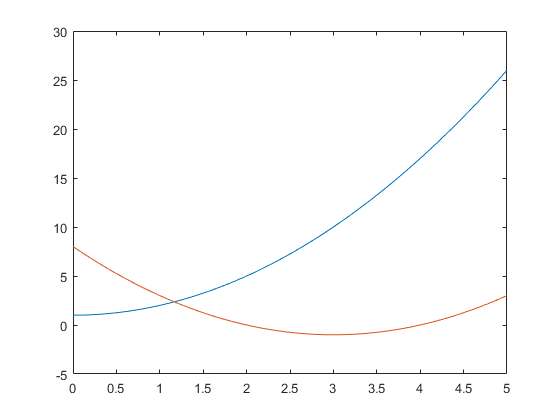
\includegraphics[width=5cm]{source/img/h4q1a}
      \end{center}
      
    \end{proof}    
  }
  \item{\textit{Lagrangian and dual function.} Plot the objective $x^{2} + 1$ versus $x$. On the same plot, show the feasible set, optimal point and value, and plot the Lagrangian $L(x, \lambda)$ versus $x$ for a few positive values of $\lambda$. Verify the lower bound property ($p^{*} \geq \inf_{x} L(x, \lambda)$ for $\lambda \geq 0$). Derive and sketch the Lagrange dual function $g$.
    \begin{proof}[\sol]
      The Lagragian for our problem is given by:
      \[
      L(x,\lambda) = (1+\lambda)x^{2} - 6\lambda x + (1 + 8\lambda)
      \]
      The graph of the feasible set is below:\\
      \begin{center}
      	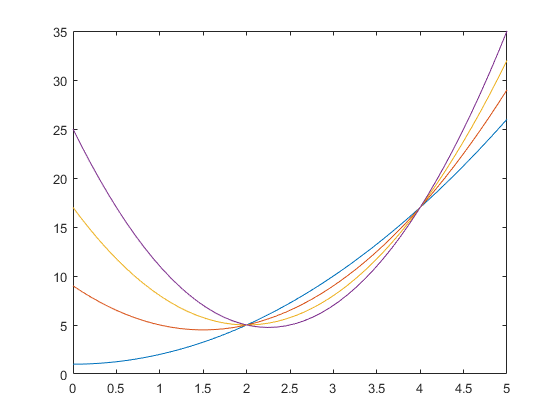
\includegraphics[width=5cm]{source/img/h4q1b}
  \end{center}


      The graph to the right shows the plot of $g(\lambda)$ with is unbounded below. Also, note that $g$ is concave and is equal to $p^{*} = 5$, when $\lambda = 2$.
      
    \end{proof}
  }
   \item{\textit{Lagrange dual problem.} State the dual problem, and verify that it is a concave maximization problem. Find the dual optimal value and dual optimal solution $\lambda^{*}$. Does strong duality hold?
     \begin{proof}[\sol]
       The dual problem is given by:
       \begin{eqnarray*}
         \mbox{maximize } & -9\lambda^{2}/(1+\lambda) + 8\lambda + 1\\
         \mbox{subject to } & \lambda \geq 0
       \end{eqnarray*}
       From (b) we noted that the max occurs when $\lambda = 2$, with a solution $d^{*} = 5$.  Therefore, strong duality holds for our problem.
    \end{proof}
   }
   \item{\textit{Sensitivity analysis.} Let $p^{*}(u)$ denote the optimal value of the problem
       \begin{eqnarray*}
    \mbox{minimize} & x^{2} + 1\\
    \mbox{subject to} & (x-2)(x-4) \leq u
       \end{eqnarray*}
       as a function of the parameter $u$. Plot $p^{*}(u)$. Verify that $\dfrac{dp^{*}(0)}{du} = -\lambda^{*}$.
       \begin{proof}[\sol]
         Similar to our dual problem, our problem is infeasible if $u < -1$,
         This is due to the fact the the $\inf_{x} x^{2} - 6x + 8) = -1$. Solving, our equation for when $u \geq -1$, we will find the roots to our equation and determine the interval for where we have a feasible set.  This will give the interval:
         \[
         \left [ 3 - \sqrt{1 + u}, 3 + \sqrt{1 + u}\right]
         \]
         Now, our optimal point will occur in the feasible reagion and should occur at $x^{*} = 3 - \sqrt{1 + u}$. So, for $p^{*}$ we have:
         \[
         p^{*} =
      \begin{cases}
          \infty& u < -1\\ 
          11 + u - 6 \sqrt{1+u} & -1 \leq u < 8\\
          1 & u \geq 8
      \end{cases}
      \]
      Now, if we differentiate $p^{*}$ we get:
      \[
      \frac{dp^{*}(0)}{du} = 2 = -\lambda
      \]
         
    \end{proof}
   }
  \end{enumerate}
